\documentclass[oneside, 12pt]{book}
\usepackage{icdthesisUTF}
\usepackage{tabularx} 
\usepackage{epsfig}

\renewcommand{\thesistitle}{Ανάπτυξη eργαλείου για την σχεδίαση παιχνιδιών με την βοήθεια υπο-λογιστή }
\renewcommand{\thesisauthor}{Γιώργου Μιχαηλίδη}
\renewcommand{\thesisauthorabbrv}{Γ. Μιχαηλίδης}
\renewcommand{\thesisauthorinitials}{ΓΜ}
\renewcommand{\thesissupervisor}{Δρ. Νικόλαος Πεταλίδης. Επιστημονικός Συνεργάτης}
\renewcommand{\thesismonth}{Φεβρουάριος}
\renewcommand{\thesisyear}{2016}

% Η βιβλιογραφία
\addbibresource{testUTF.bib}

\begin{document}
	
	\Titlepage
	\Declarationpage
	
	\begin{Abstract}
		Τα πρώτα ηλεκτρονικά παιχνίδια είχαν γραφτεί εξ'ολοκλήρου σε υλισμικό. Από τότε, οι κάρτες γραφικών και οι μικροεπεξεργαστές βελτιώθηκαν, δημιουργήθηκαν κονσόλες φτιαγμένες αποκλειστικά για ηλεκτρονικά παιχνίδια, με ειδικά χειριστήρια τα οποία σου προσφέρουν διαφορετικές εμπειρίες.
		Η διαδικασία ανάπτυξης λογισμικού είναι ακριβή και ο σχεδιασμός γίνεται όλο πιο σύνθετος και περίπλοκος. Τα έργα γίνονται όλο πιο απαιτητικά και δαπανηρά. Δημιουργήθηκε η ανάγκη για ένα εργαλείο το οποίο να παρέχει ένα ομοιογενές περιβάλλον για την ανάπτυξη σύνθετων έργων. 
		Ένα CASE (Computer Aided Software Engineering) tool είναι ένα λογισμικό-εργαλείο το οποίο απλοποιεί τον κύκλο ανάπτυξης ενός λογισμικού. 
		Στο τομέα του σχεδιασμού παιχνιδιών το πιο διαδεδομένο CASE tool είναι η μηχανή γραφικών. Μια μηχανή γραφικών είναι μια σουίτα από επαναχρησιμοποιήσιμα οπτικά εργαλεία τα οποία βρίσκονται σε ένα ενιαίο περιβάλλον.
		Σκοπός της πτυχιακής είναι να αναγνωριστούν μοτίβα και τεχνικές δημιουργίας παιχνιδιών, ώστε να δημιουργηθεί ένα εργαλείο το οποίο να το προσεγγίζει από υψηλό επίπεδο με αφαιρέσεις για εύκολη μοντελοποίηση και αυτοματοποίηση κατά τη δημιουργία.
	\end{Abstract}
	\tableofcontents
	\listoftables
	\listoffigures
	
	\begin{Preface}
		Εδώ μπορεί να μπει πρόλογος. (Δεν είναι απαραίτητο).
	\end{Preface}
	
	\begin{Acknowledgement}
		Ευχαριστίες (στο μπαμπά, στη μαμά, κτλ)
	\end{Acknowledgement}
	
	\begin{Definitions}
		Ορισμοί εννοιών που μπορεί να είναι χρήσιμοι. Για παράδειγμα:	
		\begin{description}
			\item [\LaTeX] Σύστημα στοιχειοθεσίας κειμένων
		\end{description}
		
	\end{Definitions}
	
	\chapter{Εισαγωγή}
			
		\leftmark\rightmark
		\section{Η τυπογραφία σήμερα}
		Αυτή είναι η αναφορά σε ένα άρθρο περιοδικού:\citep{Schmidt98}.Αυτή
		είναι η αναφορά σε ένα βιβλίο:\citep{goosens93}. Αυτή είναι η αναφορά
		σε ένα ελληνικό βιβλίο:\citep{Chatzigeorgiou05}. Βιβλίο στα ελληνικά
		με ξένο συγγραφέα:\citep{Sommerville09}. Άρθρο σε
		συνέδριο~\citep{4343930}. 
		
		Τέλος αναφορά σε ιστοσελίδα:~\citep{Wikipedia_BibTeX}.
		
		Εδώ αναφερόμαστε στo σχήμα~\ref{fig:image1}:
		\begin{figure}[h]
			\centering
			
\includegraphics[width=35mm]{lion.png}
			\caption{Παράδειγμα εικόνας}
			\label{fig:image1}
		\end{figure}
		
		και εδώ στον πίνακα~\ref{tab:table1}:
		\begin{table}[h]
			\centering
			\caption{Παράδειγμα πίνακα}
			\begin{tabularx}{\linewidth}[h]{|XXX|}%
				\hline
				\hline
				Κίνητρα & Παραδείγματα ευρημάτων & Αριθμός μελετών\\
				\hline
				Ταύτιση με το έργο & Ξεκάθαροι στόχοι &20\\
				Καλό management & Ομαδικότητα &16\\
				Συμμετοχή υπαλλήλων & Συμμετοχή στις αποφάσεις&16\\
				Προοπτικές εξέλιξης & Προοπτικές προαγωγής&15\\
				Ποικιλία στην εργασία & Καλή χρήση ικανοτήτων& 14\\
				Αίσθηση του να ανήκεις κάπου& Υποστηρικτικές σχέσεις&14\\
				Αμοιβές και κίνητρα & Αυξημένος μισθός& 14\\
				\hline
				\hline
			\end{tabularx}
			\label{tab:table1}
		\end{table}
		\appendix
	
		
	\chapter{Μηχανές γραφικών}
	
	\chapter{Διαδικτύωση}
		Διαδικτύωση στα ηλεκτρονικά παιχνίδια, είναι η δυνατότητα περισσότερων από ένα φυσικό άτομο να μοιράζονται και να αλληλεπιδρούν στο ίδιο εικονικό περιβάλλον. 
		
		\subsection{Τεχνικές}
		Περιγραφή τεχνικών

		\begin{itemize}	
			\item Client-server model: στο οποίο ο client απλά κάνει render και το μεγαλύτερο κομμάτι της λογικής τρέχει στον server. Ο server στέλνει οδηγίες στον client για το τι να κάνει render και ο client απλά υπακούει.
			\item Client on top of server model: ο client είναι και server, δηλαδή οι μηχανές που έχουν τον client έχουν και τον server.
			\item Peer-to-peer: οι μηχανές συμπεριφέρονται μερικώς ως clients και μερικώς ως servers, δηλαδή έχουν και στοιχεία λογικής και επεξεργασίας.
		\end{itemize}
			
		\section{Αρχιτεκτονική}		
			\begin{figure}[h]
				\centering
				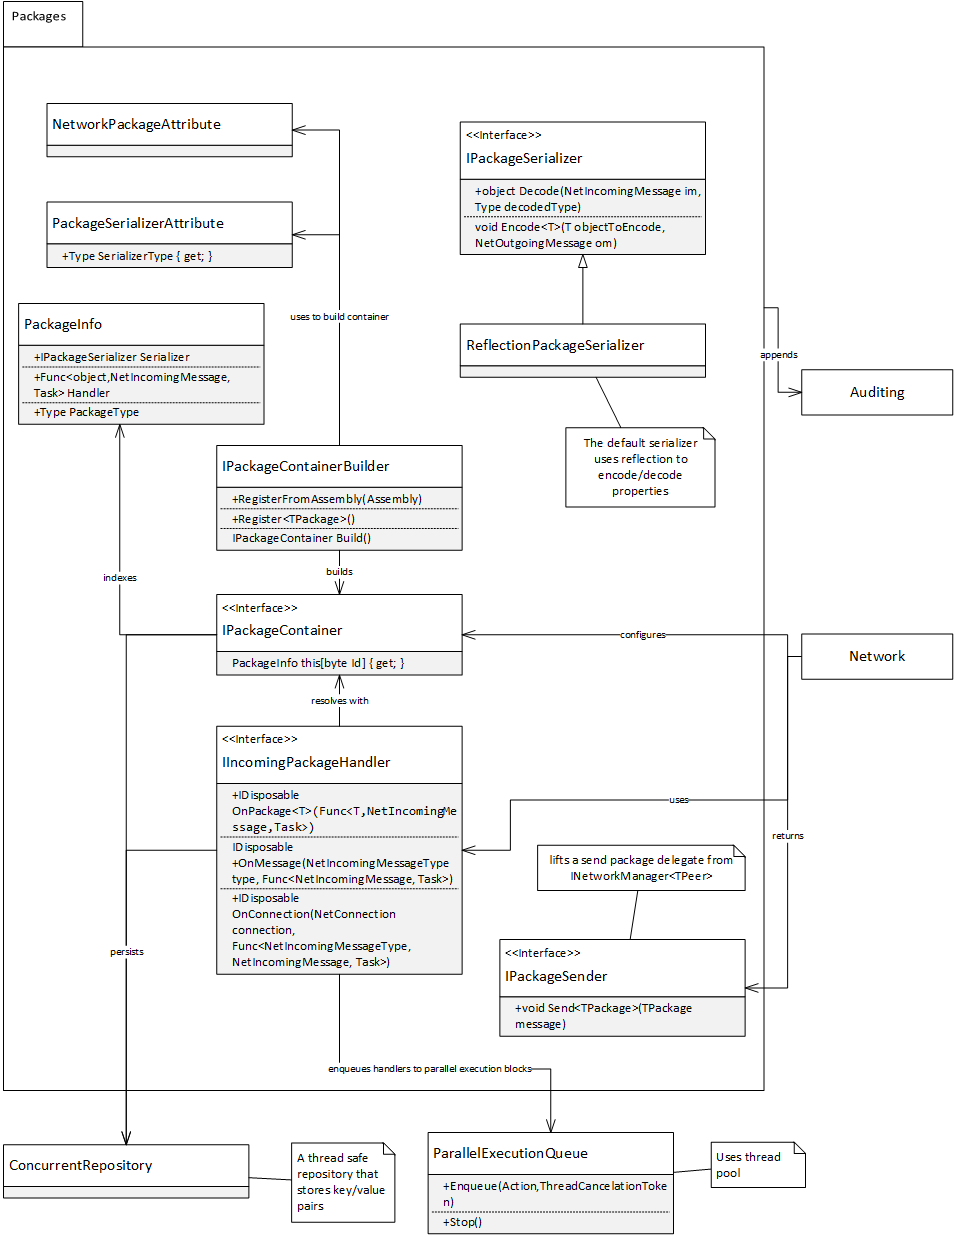
\includegraphics[width=165mm]{Images/network_architecture_packages}
				\caption{Network Packages Module}
				\label{network_packages}
			\end{figure}
			
			
			
			\subsection{Ανταλλαγή μηνυμάτων}
			
			\subsection{Client}	
			
			\subsection{Server}	

	\chapter{Game Host}
	\section{Αρχιτεκτονική}		
	
	\chapter{Περίληψη}
	
	\begin{Glossary}
		Το γλωσσάρι μπορεί να είναι χρήσιμο αν χρησιμοποιείτε πολλά ακρώνυμα
		και συντομογραφίες. Για παράδειγμα
		\begin{description}
			\item[TCP]Transmission Control Protocol
		\end{description}
	\end{Glossary}
	
	\printbibliography
	%\lastpageinfo
	




\end{document}
